\documentclass{beamer}
\usetheme{Berlin}
\usecolortheme{beaver}
\usepackage{graphicx}
\usepackage[export]{adjustbox}
\usepackage{tikz}
\usetikzlibrary{arrows}
\usepackage{amsmath}
\usepackage{lmodern}% http://ctan.org/pkg/lm
\usepackage{mathtools}

\title{Chapters 9.3-9}
\subtitle{}
\author[Riccardo \and Eren]{Riccardo~Miccini\inst{1} \and Eren~Can~\inst{1}}
\institute[DTU]
{
	\inst{1}
	Technical University of Denmark\\
	Digital Communication
}
\date{\today}
\subject{Digital Communication}

\tikzstyle{int}=[draw, fill=blue!20]
\tikzstyle{every node}=[font=\tiny]

\begin{document}
\frame{\titlepage}

% ch 9.3
\begin{frame}
	\frametitle{Modulation Schemes not Requiring Coherent References}
	\begin{itemize}
		\item In this section, now we consider two modulation schemes that you do not need to require the acquisition of  a local reference signal in phase coherence with the received carrier. 
	\end{itemize}
\end{frame}

\begin{frame}
	\frametitle{Differential Phase-Shift Keying  (DPSK)}
	\begin{itemize}
		\item The implementation of a such a scheme presupposes two things;
		\begin{enumerate}
		\item The unknown phase perturbation on the signal varies  slowly that the phase is constant from one signalling interval to next.
		\item  The phase during a given signalling interval bears a known relationship to the phase during the preceding signalling interval bears a known relationship to the phase during the preceding signalling interval.
	\end{enumerate}
	\end{itemize}
	\begin{figure}
	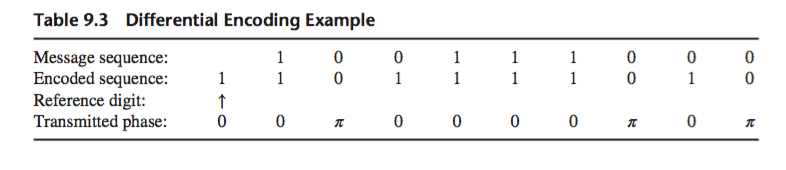
\includegraphics[width=0.8\textwidth]{9_3.png}
	\end{figure}
\end{frame}

\begin{frame}
	\frametitle{Differential Encoding Message Sequence}
	\begin{itemize}
		\item An arbitrary reference binary digit is being selected as an initial digit of the sequence
		\item For each digit , the present digit used as a reference
		\item 0 in the message sequence is encoded as  a transition from state of reference digit to the opposite state in the encoded message sequence
		\item 1 encoded as no change of state
	\end{itemize}
	\begin{figure}
		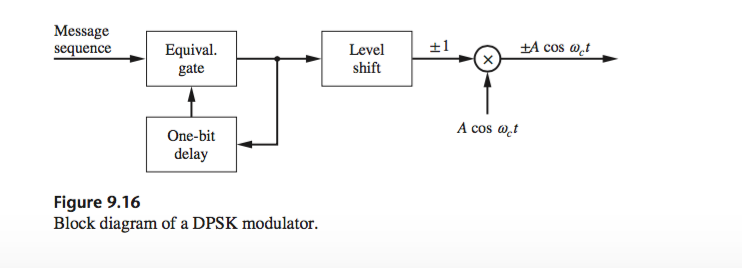
\includegraphics[width=0.8\textwidth]{9_3_1.png} \\
	\end{figure}
\end{frame}

\begin{frame}
\frametitle{Figure for Differential Encoding Message Sequence}
	\begin{figure}
		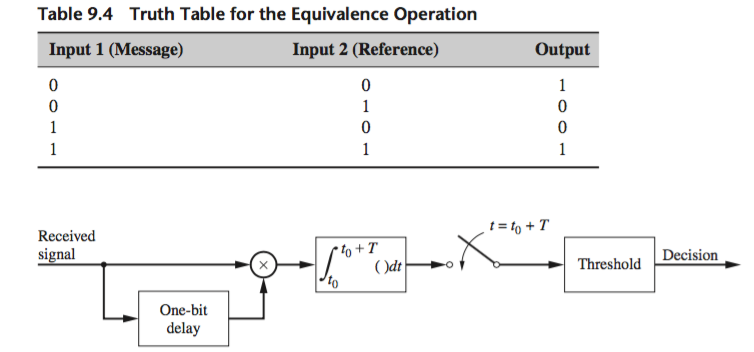
\includegraphics[width=\textwidth]{9_4_1.png}
	\end{figure}
\end{frame}		

\begin{frame}
	\frametitle{Differential Encoding Message Sequence}
	\begin{itemize}
		\item After the reference bit and plus the first encoded bit, signal input become $S_1=A \cos(\omega_c) t$ and $R_1=A*cos(w_c)*t$
		\item Than the output correlator is; $v_1= \int_{0}^{T} A^2 \cos^2(\omega_c t) dt$ which eventually become $\frac{1}{2} A^2 T$
		\item The optimum detector for binary will become  $l= x_k x_k-1 +y_k y_k-1$
		\item Without a loss of of generality, we can choose $\theta=0$; we found outputs at $t=0$ to be:
			\begin{itemize}
			\item $x_0= \frac{A T}{2}+n_1$ and $y_0=n_3$ and where $n_1=  \int_{-T}^{0} n(t) \cos^2(\omega_c t) dt$
			\item  $n_3=\int_{-T}^{0} n(t) \sin^2(\omega_c t) dt$. Similarly, at the time $t=T$, the outputs are ;
			$x_1=\frac{AT}{2}+n_2$ and $y_1=n_4$
			\item $n_2=\int_{0}^{T} n(t) \cos^2(\omega_c t) dt$
			\item $n_4=\int_{0}^{T} n(t) \sin^2(\omega_c t) dt$
			\end{itemize}
	\end{itemize}
\end{frame}

\begin{frame}
	\frametitle{Important Figure for Differential Encoding }
	\begin{figure}
		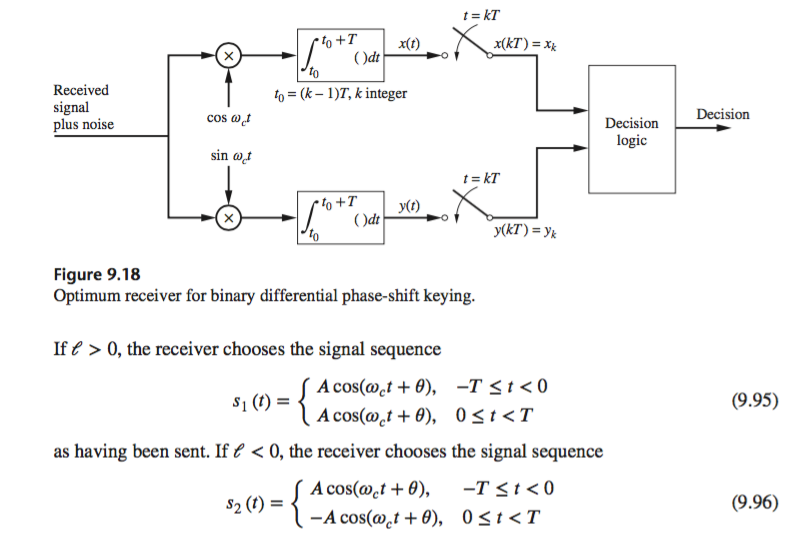
\includegraphics[width=0.8\textwidth]{9_4_2.png}
	\end{figure}
\end{frame}

\begin{frame}
	\begin{itemize}
		\item It follows as $n_1, n_2, n_3 and n_4$ are uncorrelated and zero-mean Gaussian random variables with variances $\frac{N_0 T}{4}$ and they are independent.
		\item Expression for Probability error $P_E= Pr [(\frac{A T}{2}+n_1)(\frac{A T}{2}+n_2)+n_3 n_4<0]$
		\item We can define new gaussian random variables  such as:
		$ \omega_1=\frac{n_1}{2}+\frac{n_2}{2} $ \\
		$ \omega_2=\frac{n_1}{2}-\frac{n_2}{2}  $\\
		$ \omega_3=\frac{n_3}{2}+\frac{n_4}{2}$ \\
		$ \omega_4=\frac{n_3}{2}-\frac{n_4}{2} $
	\end{itemize}
\end{frame}

\begin{frame}
	\begin{itemize}
		\item Probability can be written in terms of Gaussian variables:
		$P_E= Pr [(\frac{A T}{2}+\omega_1)^2 +(\omega_3)^2<(\omega_2^2+\omega_4^2)]$
		\item Gaussian variables will also let us define the Ricean random variables. Ricean random variable will become: $R_1=\sqrt{(\frac{AT}{2}+\omega_1)^2+\omega_3^2}$
		\item Also Rayleigh random variable will become $R_2=\sqrt{\frac{\omega_2^2}{\omega_4^2}}$
		\item If we also define the bit energy $E_b$ as $A^2 \frac{A^2 T}{2}$ will give;
		$P_E=\frac{1}{2} e^(\frac{-E_b}{N_0}$ for the optimum DPSK receiver.
		\item At the large values  $\frac{-E_b}{N_0}$ values of ;
		$P_E=Q[\sqrt{\frac{-E_b}{N_0}}]=Q[\sqrt{z}]$
	\end{itemize}
\end{frame}

\begin{frame}
	\begin{itemize}
	\item Following result obtained by using the asymptotic approximation;
	$P_E=\frac{e^(-E_b/N_0)}{2 \sqrt{\pi \frac {E_b}{N_0}}}$
	\end{itemize}
\begin{figure}
	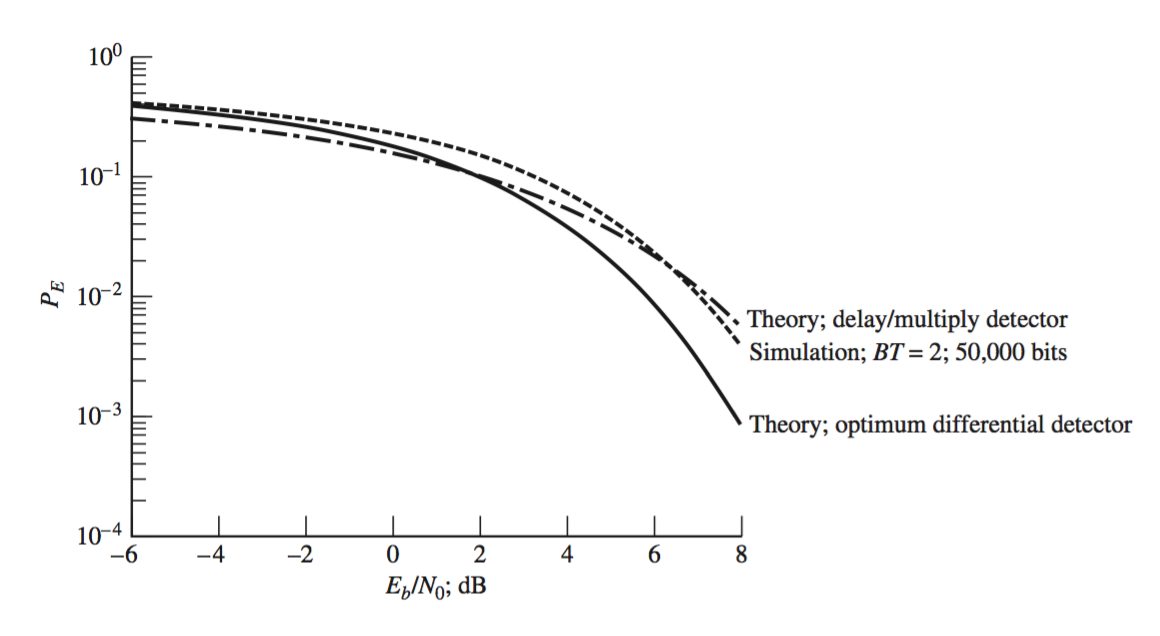
\includegraphics[width=0.8\textwidth]{9_5.png}
\end{figure}
\end{frame}
% ch 9.5
\begin{frame}
	\frametitle{Comparison of Digital Modulation Systems}
	\begin{itemize}
		\item Bit error probabilities are compared in Figure 9.22 for the modulation schemes that considered in this chapter. Note that the curve for antipodal binary PAM is identical to BPSK
		\item  Also bit error probability of antipodal PAM  becomes worse the larger M. Curves move more to the right as M gets larger
	\end{itemize}
\end{frame}

	\begin{frame}
	\frametitle{Important figure for Chapter 9}
	\begin{figure}
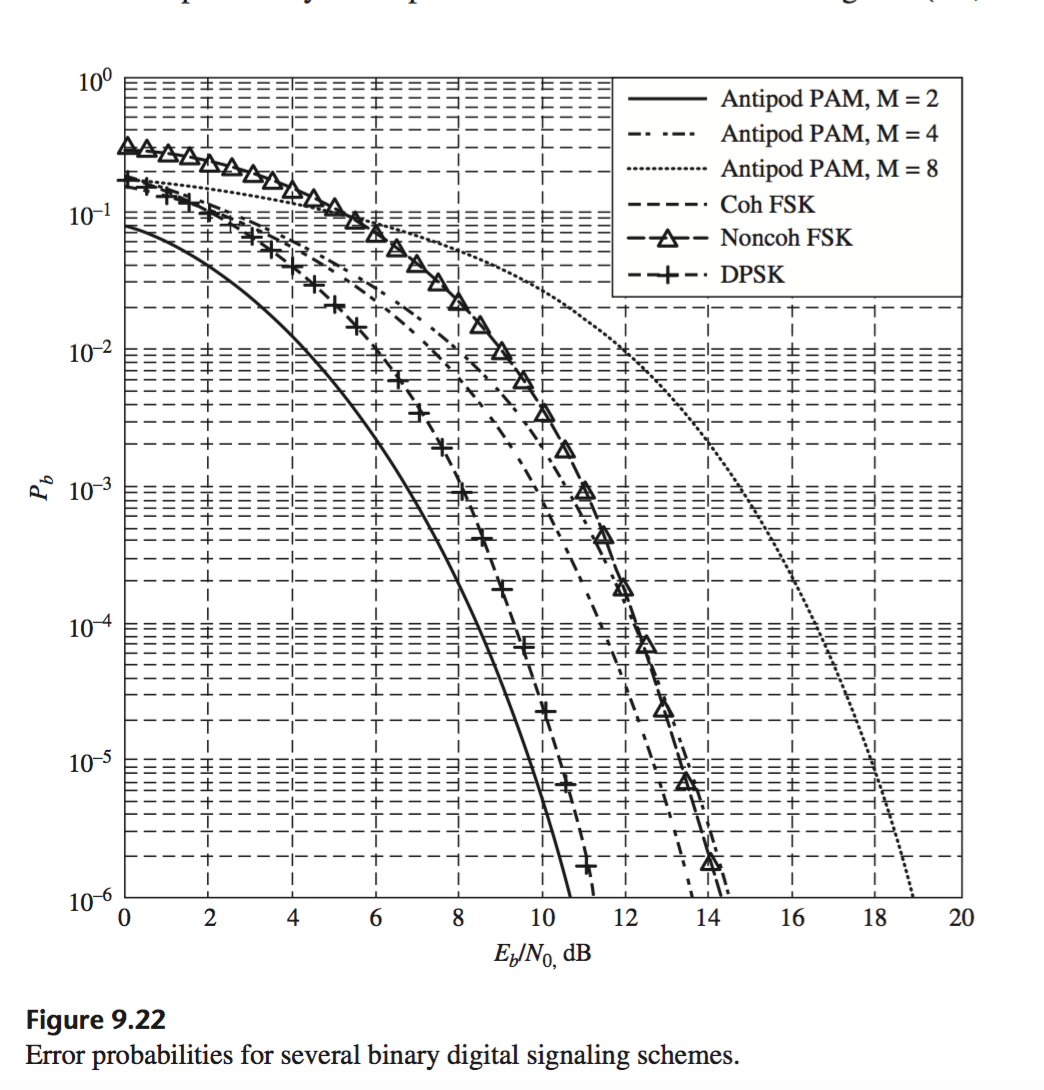
\includegraphics[width=0.5\textwidth]{9_5_1.png}
	\end{figure}
\end{frame}

\begin{frame}
	\begin{itemize}
	\item Non-coherent binary FSK and PAM with M=4 have almost identical performance at large signal-to-noise ratios.
	\item	In addition to cost and complexity implementation, there are many other considerations in choosing one type of digital data system over another.
	\item Some channels, where the channel gain, phase or when both are in effect,we use a noncoherent system may be dictated because of impossibility of establishing a coherent reference at the receiver  under such conditions. They will be referred as "fading".
	\end{itemize}
\end{frame}


% ch 9.7
\begin{frame}
	\frametitle{Multipath Interference}
	\begin{itemize}
		\item .
	\end{itemize}
\end{frame}


% ch 9.9
\begin{frame}
	\frametitle{Equalization}
	\begin{itemize}
		\item .
	\end{itemize}
\end{frame}

\begin{frame}
	\frametitle{Equalization by Zero Forcing}
	\begin{itemize}
		\item .
	\end{itemize}
\end{frame}

\begin{frame}
	\frametitle{Equalization by Minimum Mean-Squared Error}
	\begin{itemize}
		\item .
	\end{itemize}
\end{frame}

\begin{frame}
	\frametitle{Tap Weight Ajustment (LMS Algorithm)}
	\begin{itemize}
		\item .
	\end{itemize}
\end{frame}

\end{document}
